\documentclass[12pt,letterpaper]{article}
\usepackage{fullpage}
\usepackage[top=2cm, bottom=4cm, left=2.5cm, right=2.5cm]{geometry}
\usepackage{amsmath,amsthm,amsfonts,amssymb,amscd}
\usepackage{lastpage}
\usepackage{enumerate}
\usepackage{fancyhdr}
\usepackage{mathrsfs}
\usepackage{xcolor}
\usepackage{graphicx}
\usepackage{listings}
\usepackage{hyperref}
\usepackage{float}

\hypersetup{%
  colorlinks=true,
  linkcolor=blue,
  linkbordercolor={0 0 1}
}
 
\renewcommand\lstlistingname{Algorithm}
\renewcommand\lstlistlistingname{Algorithms}
\def\lstlistingautorefname{Alg.}

\lstdefinestyle{Python}{
    language        = Python,
    frame           = lines, 
    basicstyle      = \footnotesize,
    keywordstyle    = \color{blue},
    stringstyle     = \color{green},
    commentstyle    = \color{red}\ttfamily
}

\setlength{\parindent}{0.0in}
\setlength{\parskip}{0.05in}
\begin{document}

\begin{enumerate}
    \item \emph{Solution}\\
    \begin{enumerate}
        \item Graphing $f(x) = x$ and $g(x) = 2sin(x)$: \\
        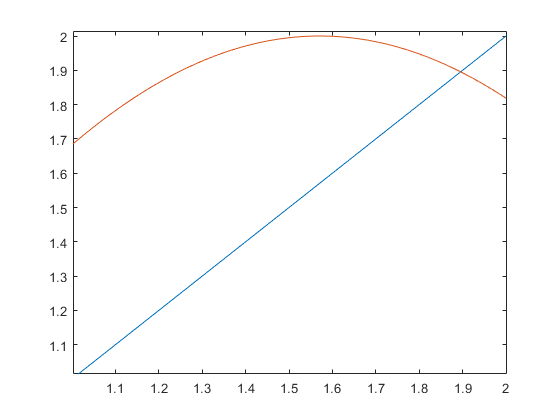
\includegraphics{number1a.png}\\
        \item 
        Using the bisection.m and the runbisection.m files, we find that the first 
        positive root is at $1.895492553710938e+00$ and converged in 16 iterations: \\
        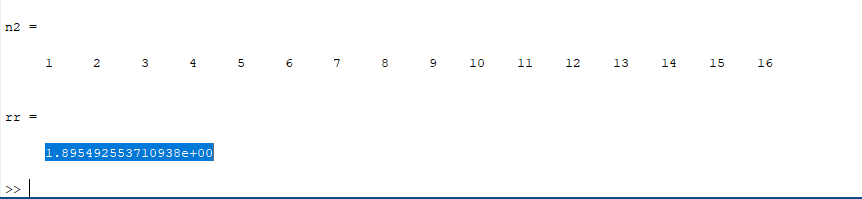
\includegraphics[scale = .7]{number1b.png}\\
    \end{enumerate}

    \item \emph{Solution.}\\
    Graphing the function: \\
    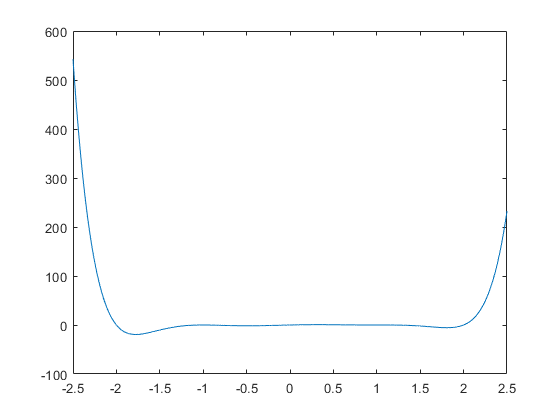
\includegraphics{number2graph.png}
    \begin{enumerate}
        \item $\left [-2.5, -1.5 \right]$\\
        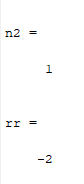
\includegraphics{2a.png}\\
        Here, the bisection method converges to -2
        \item $\left [-1.5, -0.5 \right]$\\
        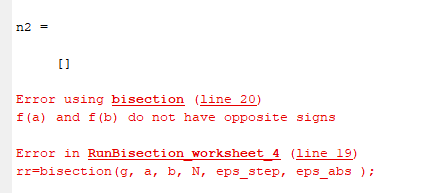
\includegraphics{2b.png}\\
        Here, the bisection did not work, as the function is negative on the whole
        interval and so $f(a)$ and $f(b)$ do not have different signs. 
        \item $\left [-0.5, 0.5 \right]$\\
        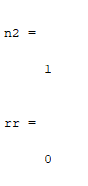
\includegraphics{2c.png}\\
        Here, the bisection method converges to 0
        \item $\left [0.5, 1.5 \right]$\\
        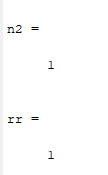
\includegraphics{2d.png}\\
        Here, the bisection method converges to 1
        \item $\left [1.5, 2.5 \right]$\\
        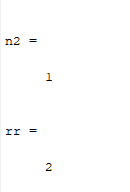
\includegraphics{2e.png}\\
        Here, the bisection method converges to 2
    \end{enumerate}
    
    \item 
    To find the number of iterations needed to achieve and approximation with 
    an accuracy of at least $10^{-3}$ , we use the equation:
    \begin{gather*}
        |p_n - p| = \frac{b-a}{2^n}\\
        10^{-3} = \frac{4-1}{2^n}\\
        2^n = 3(10^{3})\\
        \ln(2^n) = n\ln(2) = ln(3(10^3))\\
        n = \frac{\ln(3(10^3))}{\ln(2)}\\
        n \approx 11.55
    \end{gather*}
    Thus, we find it takes about 12 iterations to find an approximation with an 
    accuracy of $10^{-3}$

    When we run the bisection method on this function, we find indeed that our 
    theoretical result was spot on with our experimental result: \\
    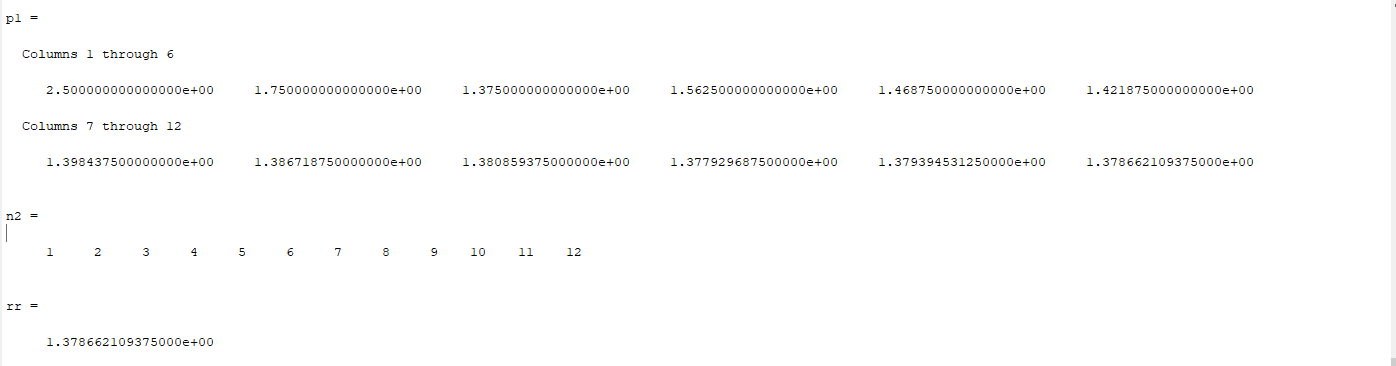
\includegraphics[scale = .5]{number3.png}

    \item 
    Using the bisection method, we find that the first two roots are $-5$ and $-3$. 
    The root where $x = 1$, however, we cannot find using the bisection method, as 
    the function does not change signs near that specific root. \\
    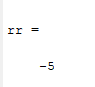
\includegraphics{4a.png}\\
    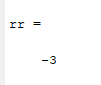
\includegraphics{4b.png}

    \item For the roots we can find with the bisection method: \\
    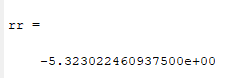
\includegraphics{5a.png}\\
    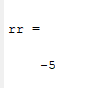
\includegraphics{5b.png}\\
    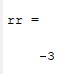
\includegraphics{5c.png}\\
    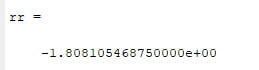
\includegraphics{5d.png}\\
    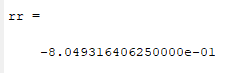
\includegraphics{5e.png}\\
    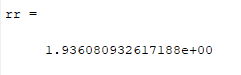
\includegraphics{5f.png}\\
    The root at $x=1$ cannot be determined by the bisection method, as there is no 
    sign change around that point. Numerical methods which require the first derivative
    would not always work, as this function is not everywhere differentiable. Since
    the function at $x=1$ is the highest point around the root, $f(1)$ would have 
    to one of the end points. Since $f(1)$ must be an endpoint, and the IVT only
    guarantees a root inside the interval, the IVT does not guarantee a root. 

\end{enumerate}

\end{document}